\documentclass[12pt]{article}
\usepackage[english]{babel}
\usepackage[utf8]{inputenc}
\usepackage{amsmath, amssymb, amsthm}
\usepackage{graphicx}
\usepackage{hyperref}
\usepackage[margin=.75in]{geometry}
\usepackage{xcolor}
\usepackage{tikz}

\newcommand{\id}{\text{id}}
\newcommand{\od}{\text{od}}

\setlength{\topmargin}{0pt}
\setlength{\headsep}{0pt}
\textheight = 600pt

\title{Graph Theory \\ Homework 12}
\author{Ben Kallus and Ryan Friedman}
\date{Due Thursday, April 8}

\begin{document}
\maketitle

\medskip\noindent\textbf{8.18} Proposition: There exists a 5-regular graph with no 1-factor.
\begin{proof}
    The graph shown below is clearly 5-regular, but has an odd number of vertices, and thus has no 1-factor.
    \begin{center}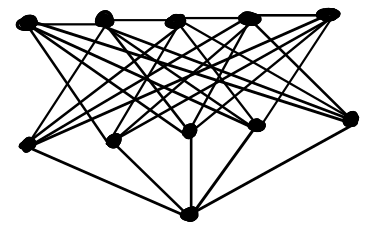
\includegraphics{pic1.png}\end{center}
\end{proof}

\newpage\noindent\textbf{8.20} Proposition: Every 3-regular graph with at most two bridges contains a 1-factor.
\begin{proof}
    Let $G$ be a 3-regular graph, and let $S \subseteq V(G)$.
    Let $G_1, \hdots, G_\ell$ denote the odd components of $G-S$, and let $G_{\ell+1}, \hdots, G_j$ denote the even components of $G-S$.
    Then, $$V(G) = G_1 \sqcup \hdots \sqcup G_{\ell} \sqcup G_{\ell+1} \hdots \sqcup G_j.$$
\end{proof}

\newpage\noindent\textbf{8.24}



\newpage\noindent\textbf{8.26}



\newpage\noindent\textbf{8.28}



\end{document}
